\documentclass[12pt, a4paper]{article}

\usepackage[T1]{fontenc}
\usepackage{courier}
\usepackage{graphicx}
\usepackage{caption}
\usepackage{mathptmx}
\usepackage{ragged2e}
\usepackage{xcolor}
\usepackage{listings}
\usepackage{enumitem}

\graphicspath{{img}}
\pagenumbering{gobble}
\date{}

\captionsetup[figure]{labelformat=empty}

\title{

  \large{\textbf{LAPORAN}}

  \large{\textbf{EKSPLORASI CARA KERJA DAN KEGUNAAN APLIKASI SERVER GNS3}}

  {\large{Diajukan untuk Memenuhi Tugas Mata Kuliah Jaringan Komputer}}

  {\vspace{1cm}}

  \normalsize{Radinal Shidiq Saragih}

  {\vspace{0.5cm}}

  \normalsize{IF C 2023}

  {\vspace{0.5cm}}

  \normalsize{5520123104}

  {\vspace{1cm}}

  {
\includegraphics[scale=1.8]{LogoFakultas.jpeg}}

  {\vspace{2cm}}

  {\large{PROGRAM STUDI TEKNIK INFORMATIKA}}

  {\large{FAKULTAS TEKNIK}}

  {\large{UNIVERSITAS SURYAKANCANA}}

  {\large{CIANJUR}}

  {\small{2024}}
}

\begin{document}
  \begin{titlepage}
    \maketitle
  \end{titlepage}

  \pagenumbering{roman}

  \begin{center}
    \section*{KATA PENGANTAR}
  \end{center}

  \setcounter{section}{1}

  \setcounter{subsection}{0}

  \addcontentsline{toc}{section}{KATA PENGANTAR}{}

  \vspace{1cm}


  Puji syukur saya panjatkan kepada Tuhan Yang Maha Esa, atas segala rahmat dan
  karunia-Nya, sehingga saya dapat menyelesaikan laporan ini yang berjudul
  "Eksplorasi Cara Kerja dan Kegunaan Aplikasi Server GNS-3".
  Laporan ini disusun untuk memenuhi salah satu tugas dalam mata kuliah
  Jaringan Komputer.


  GNS-3 (Graphical Network Simulator-3) merupakan salah satu aplikasi
  simulasi jaringan yang sangat bermanfaat bagi para profesional IT dan mahasiswa
  yang belajar tentang jaringan komputer. Dalam laporan ini, saya akan membahas
  cara kerja aplikasi GNS-3, fitur-fitur yang dimilikinya, serta kegunaannya
  dalam simulasi jaringan yang kompleks.


  Saya mengucapkan terima kasih kepada semua pihak yang telah memberikan dukungan
  dan bantuan dalam penyusunan laporan ini. Semoga laporan ini bermanfaat dan
  dapat memberikan wawasan baru bagi pembaca.

  \vspace{1cm}

  \begin{flushright}
    Cianjur, September 2024

    \vspace{0.5cm}

    Penulis
  \end{flushright}

  \newpage

  \renewcommand\contentsname {\Large{\textbf{DAFTAR ISI}} }

  \begin{center}
  \tableofcontents
  \end{center}
  \addcontentsline{toc}{section}{DAFTAR ISI}{}

  \newpage
  
  \pagenumbering{arabic}

  \begin{center}
    \large{\textbf{BAB I}}

    \section*{PENDAHULUAN}
  \end{center}
  \addcontentsline{toc}{section}{BAB I PENDAHULUAN}{}

  \vspace{1cm}

    \subsection{Latar Belakang}

  Di era industri 4.0, teknologi jaringan telah bagian penting dari
  kehidupan tiap orang, dengan eratnya terintegrasi teknologi
  jaringan dikehidupan tiap orang, seperti yang dinyatakan
  oleh Ambarwati dan Fauzi, ``\emph{Jaringan komputer adalah
  fondasi utama bagi perkembangan teknologi informasi yang memungkinkan komunikasi
  cepat dan efisien}`` (Ambarwati \& Fauzi, 2019). Maka para profesional
  di bidang jaringan komputer pun dipaksa untuk dapat beradaptasi cepat
  agar tetap relevan.

  GNS-3 menyediakan sebuah kesempatan bagi siapapun agar dapat
  mengembangkan ilmu dan bereksplorasi di bidang jaringan komputer tentunya
  tanpa harus mengeluarkan biaya yang besar untuk dapat membeli alat-alat
  jaringan fisik secara langsung.

    \subsection{Rumusan Masalah}

      Adapun rumusan masalah yang akan dibahas dalam laporan ini, antara lain

      \begin{enumerate}[label=\arabic*.]
        \item Apa yang dimaksud dengan GNS-3?
        \item Apa saja kegunaan dan fitur yang dimiliki GNS-3?
        \item Apa saja software pendukung GNS-3
        \item Bagaimana cara membangun simulasi jaringan komputer dalam GNS-3?
      \end{enumerate}

    \subsection{Tujuan}

      Adapun yang menjadi tujuan dari laporan ini, yaitu

      \begin{enumerate}[label=\arabic*.]
        \item Memberi pemahaman tentang GNS-3
        \item Mengetahui cara pemakaian dan fitur yang dimiliki.
        \item Menyadari potensi pengembangan ilmu yang diberikan GNS-3
      \end{enumerate}

  \newpage

  \begin{center}
    \large{\textbf{BAB II}}

    \section*{PEMBAHASAN}
  \end{center}
  \addcontentsline{toc}{section}{BAB II PEMBAHASAN}{}

  \vspace{1cm}


    \subsection{Deskripsi GNS-3}

      \begin{figure}[h]
          \centering
          
\includegraphics[scale=0.50]{GNS3LOGO.png}
          \caption{\small{Logo GNS-3}}
      \end{figure}

  Aplikasi GNS-3 (Graphical Network Simulator-3) adalah simulator jaringan komputer
  open-source yang lahir dari hasil karya kolaboratif para ahli 
  jaringan komputer. GNS-3 berfungsi untuk mensimulasikan berbagai alat atau mesin
  komputer yang bekerja sama untuk membentuk suatu sistem jaringan.

  GNS-3 dapat mensimulasikan perangkat lunak dari berbagai vendor router, switch, dan hub
  seperti Cisco, MikroTik, Juniper, dan lain-lain. Selain itu, GNS-3 juga dapat mengintegrasikan
  mesin-mesin virtualisasi ke dalam sistem yang ia simulasikan.

  Karena kemampuannya untuk membentuk simulasi topologi atau sistem jaringan yang
  kompleks dan realistis, aplikasi ini sering digunakan sebagai alat pembelajaran
  para pemula agar memahami fundamental jaringan, serta sebagai alat latihan oleh
  para ahli yang ingin memperdalam pengetahuan mereka.

    \subsection{User Interface GNS-3}

      GNS-3 menyajikan graphical interface yang cukup komprehensif, hingga
      dapat dengan mudah mevisualisasi sebuah jaringan secara langsung.

      \begin{figure}[h]
          \centering
          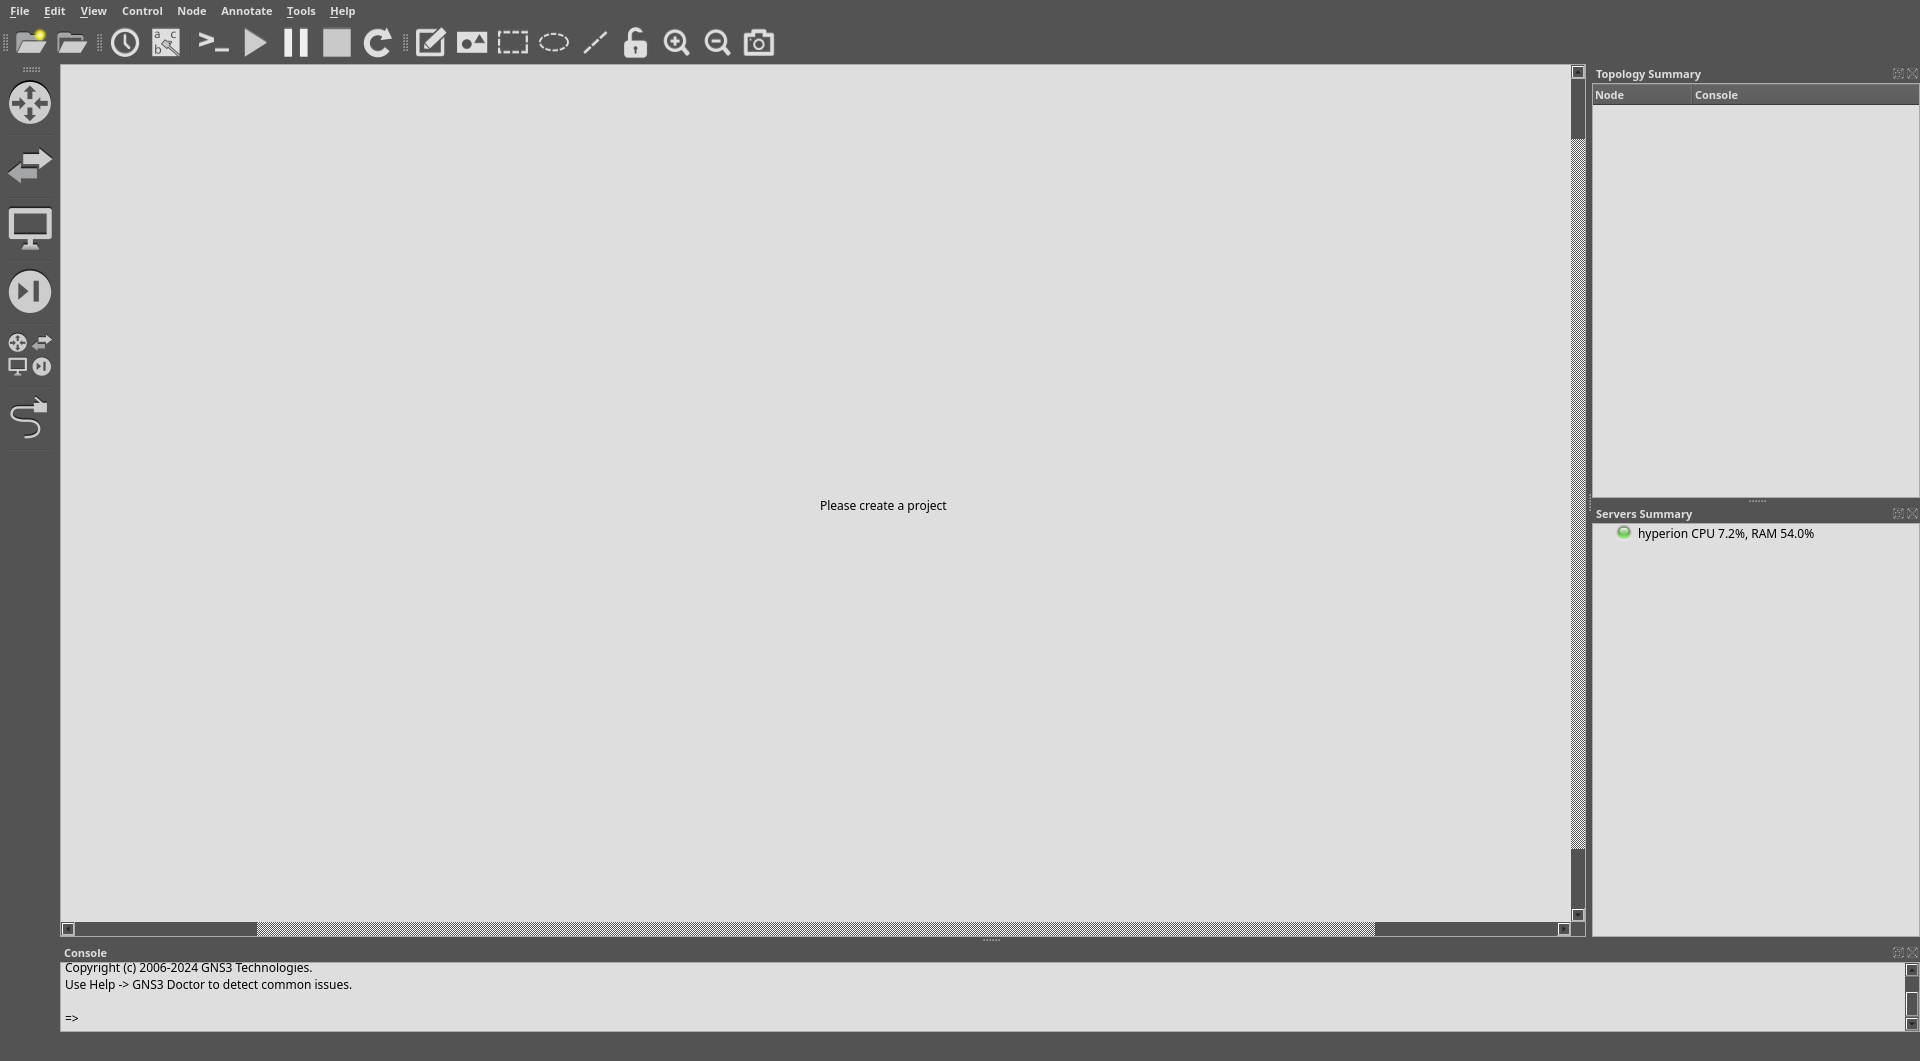
\includegraphics[scale=0.12]{GUIGNS3.png}
          \caption{\small{Tampilan Utama GNS-3}}
      \end{figure}

      Didalam tampilan aplikasi GNS-3 terdapat beberapa bagian, yaitu.

      \begin{enumerate}[label=\arabic*.]

        \item Workspace

          Workspace adalah area dimana semua device atau node akan diletakan
          dan dihubungkan.

          \begin{figure}[h]
              \centering
              \includegraphics[scale=0.12]{GNS3\_WORKSPACE.jpg}
              \caption{\small{Workspace GNS-3}}
          \end{figure}

        \item Topology Summary

          Topology Summary akan memperlihatkan informasi mengenai tiap node
          yang dibuat, mulai dari status, serta informasi mengenai koneksi
          tiap device.

          \begin{figure}[h]
              \centering
              \includegraphics[scale=0.12]{GNS3\_TOPOLOGISUM.jpg}
              \caption{\small{Topology Summary GNS-3}}
          \end{figure}

        \item Server Summary

          Server Summary akan memperlihatkan informasi mengenai tiap server
          yang terhubung, mulai dari status hingga pemakaian sumber daya.

          \begin{figure}[h]
              \centering
              \includegraphics[scale=0.12]{GNS3\_SERVERSUM.jpg}
              \caption{\small{Server Summary GNS-3}}
          \end{figure}

        \item Console

          Console akan memperlihatkan berbagai masalah atau error yang dialami
          device yang terhubung dalam GNS-3, informasi tentang error akan memudahkan
          untuk meng-troubleshoot error tersebut.

          \begin{figure}[h]
              \centering
              \includegraphics[scale=0.12]{GNS3\_CONSOLE.jpg}
              \caption{\small{Console GNS-3}}
          \end{figure}

        \newpage

        \item Device Toolbar

          Device Toolbar menyimpan berbagai device yang dapat digunakan didalam
          GNS-3, mulai dari Router, Switch, Mesin Virtual, VPCS, dan lain sebagainya.

          \begin{figure}[h]
              \centering
              \includegraphics[scale=0.12]{GNS3\_DEVICETOOLBAR.jpg}
              \caption{\small{Device Toolbar GNS-3}}
          \end{figure}

        \item GNS3 Toolbar

          Toolbar memiliki beberapa tombol untuk mengendalikan sebuah device ataupun
          seluruhnya, serta untuk memberikan deskripsi-deskripsi tambahan pada Workspace.

          \begin{figure}[h]
              \centering
              \includegraphics[scale=0.12]{GNS3\_TOOLBAR.jpg}
              \caption{\small{Device Toolbar GNS-3}}
          \end{figure}


      \end{enumerate}

    \subsection{Instalasi GNS-3 di Fedora Linux}

      Aplikasi GNS-3 ini dirilis sebagai aplikasi cross-platform jadi dapat
      dipasang di sistem operasi manapun, mulai dari windows, mac-os dan
      juga linux.

      Untuk berikut adalah langkah-langkah yang dapat diikuti untuk menginstal
      di Sistem Operasi Linux, tepatnya Fedora Linux.

      \begin{figure}[h]
          \centering
          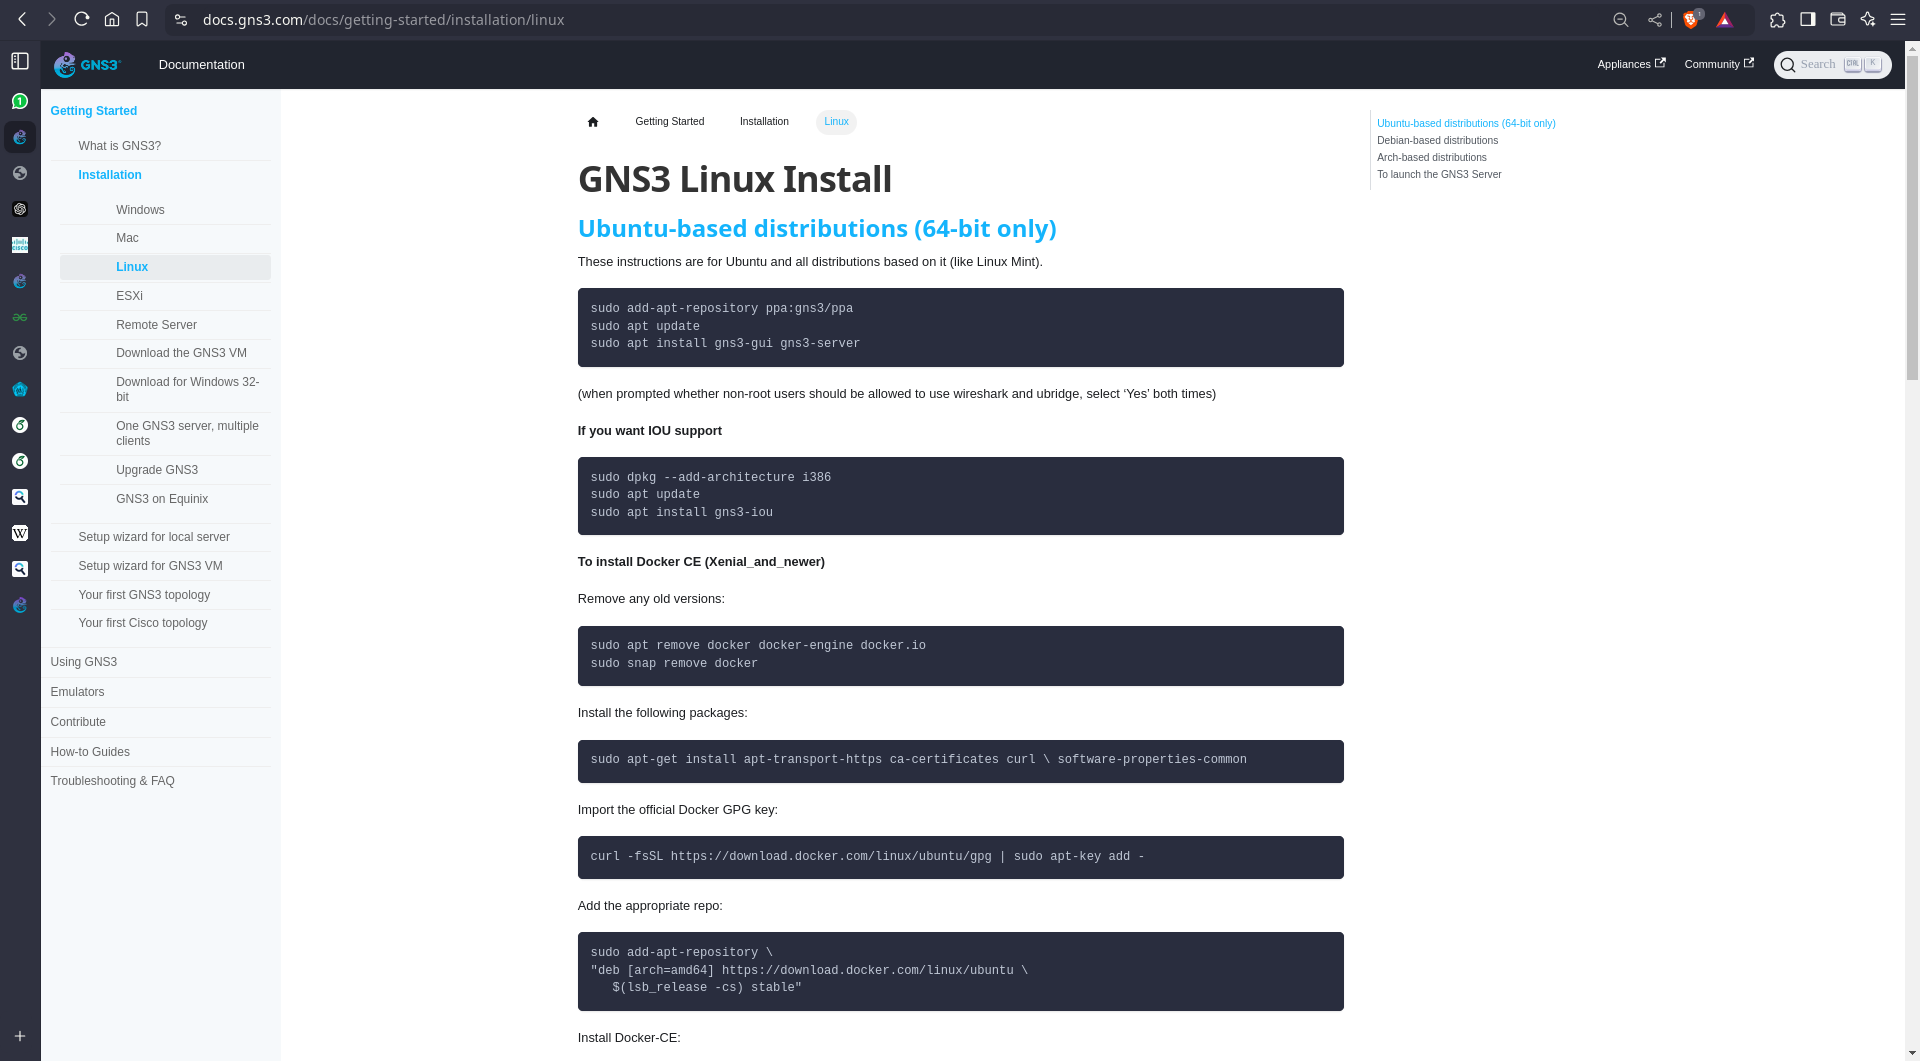
\includegraphics[scale=0.12]{LINUXINSTALLMANUAL.png}
          \caption{\small{Halaman Dokumentasi Instalasi di Linux}}
      \end{figure}

      Didalam halaman dokumentasi linux, akan diberi langkah-langkah untuk 
      dapat menginstal GNS-3 di berbagai distro linux.

      Namun, untuk Fedora Linux, di halaman unduh GNS-3 tidak akan ditemui penjelasan
      tentang instalasi, namun untungnya di dalam repository fedora sudah disediakan
      binary nya siap untuk diinstall.

      \begin{figure}[h]
          \centering
          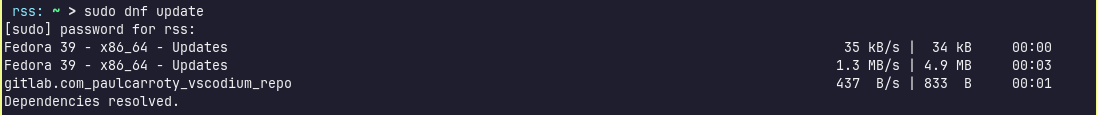
\includegraphics[scale=0.15]{FEDORAREPOSYNC.png}
          \caption{\small{Update Repository Fedora Linux}}
      \end{figure}

      Pertama yang perlu dilakukan adalah untuk memastikan apa repository fedora
      perlu update atau pembaruan index, jadi buka terminal bash lalu
      masukan perintah.
      
      \$ sudo dnf update

      Setelah repository telah diperbaruhi, baru bisa dimulai instalasi dengan
      perintah.

      \$ sudo dnf install gns3-server gns3-gui

      Perintah ini akan mengunduh dan menginstall server serta graphical interface,
      GNS-3.

      Namun tidak selesai dengan itu, setelah menginstal gns-3 perlu juga menginstall
      komponen-komponen tambahan agar dapat membangun simulasi di dalam GNS-3 nantinya.

      \subsection{Instalasi Komponen GNS-3 di Fedora Linux}

      Aplikasi GNS-3 untuk dapat mesimulasikan sebuah jaringan utuh, 
      memerlukan beberapa komponen tambahan, berikut beberapa komponen
      tersebut dan cara menginstallnya di Fedora Linux.

      \begin{enumerate}[label=\arabic*.]
        \item Dynamips

          Dalam Buku The Book of GNS3, dijelaskan bahwa ``\emph{Dynamips is the
          core component of GNS3 that emulates Cisco router hardware.
          It allows users to run Cisco IOS on a personal computer by mimicking
          the hardware architecture of real Cisco routers. This capability
          is crucial for building and testing network topologies without the
          need for physical devices, making Dynamips a key part of any network
          simulation involving Cisco devices}`` (Neumann, 2021).

          Dari kutipan tersebut dapat disimpulkan Dynamips adalah aplikasi yang
          digunakan GNS-3 untuk mengemulasikan hardware milik Cisco,
          aplikasi ini akan mengemulasikan hardware 
          hingga software router, switch, hub, dan lain sebagainya yang di
          import kedalam gns-3 dapat dijalankan.

          Untuk menginstal Dynamips di fedora linux dapat dilakukan dengan
          perintah terminal yaitu.

          \$ sudo dnf install dynamips

        \item Wireshark

          Dalam buku The Book of GNS3, dijelaskan apa itu Wireshark, yaitu.
          ``\emph{Wireshark is an essential tool integrated within GNS3 for capturing
          and analyzing network traffic. It allows users to inspect
          data flowing through a network at a granular level, providing
          deep insights into the behavior of protocols and network devices.
          This makes Wireshark invaluable for both troubleshooting and learning
          about network operations}`` (Neumann, 2021).

          Wireshark adalah aplikasi untuk menganalisis network traffic.
          GNS-3 akan menggunakan aplikasi ini untuk menganalisis topologi 
          jaringan yang dibangun didalamnya, sehingga besaran aktifitas
          jaringan dapat dilihat menggunakan alat ini.

          Untuk menginstal Wireshark di fedora linux dapat dilakukan dengan
          perintah terminal yaitu.

          \$ sudo dnf install wireshark

        \item VPCS

          Dalam buku The Book of GNS3, dijelaskan apa itu VPCS, yaitu.
          ``\emph{VPCS (Virtual PC Simulator) is a lightweight virtual machine
          used within GNS3 to simulate basic network hosts. It allows
          users to emulate simple PC endpoints that can send and receive
          pings or traceroutes, making it useful for testing basic connectivity
          and IP configurations in simulated networks without consuming excessive
          system resources}`` (Neumann, 2021).

          Jadi VPCS adalah aplikasi yang digunakan didalam gns-3 untuk mengsimulasi
          network traffic, jadi dapat digunakan untuk mengsimulasikan
          jaringan yang kompleks dan besar dengan pemakaian user yang cukup
          besar, hingga pada dasarnya VPSC adalah simulasi ringan dari sebuah
          mesin komputer.

          Untuk VPCS tidak akan ditemui didalam repository fedora linux, namun
          dapat dengan mudah menginstallnya secara manual melalui repository 
          github vpcs yang dimaintain oleh tim developer GNS-3 sendiri, karena
          repository project yang original sudah tidak lagi ada.

          Pertama buka halaman repository project vpcs di github yang ada
          pada url, https://github.com/GNS3/vpcs.

          \begin{figure}[h]
              \centering
              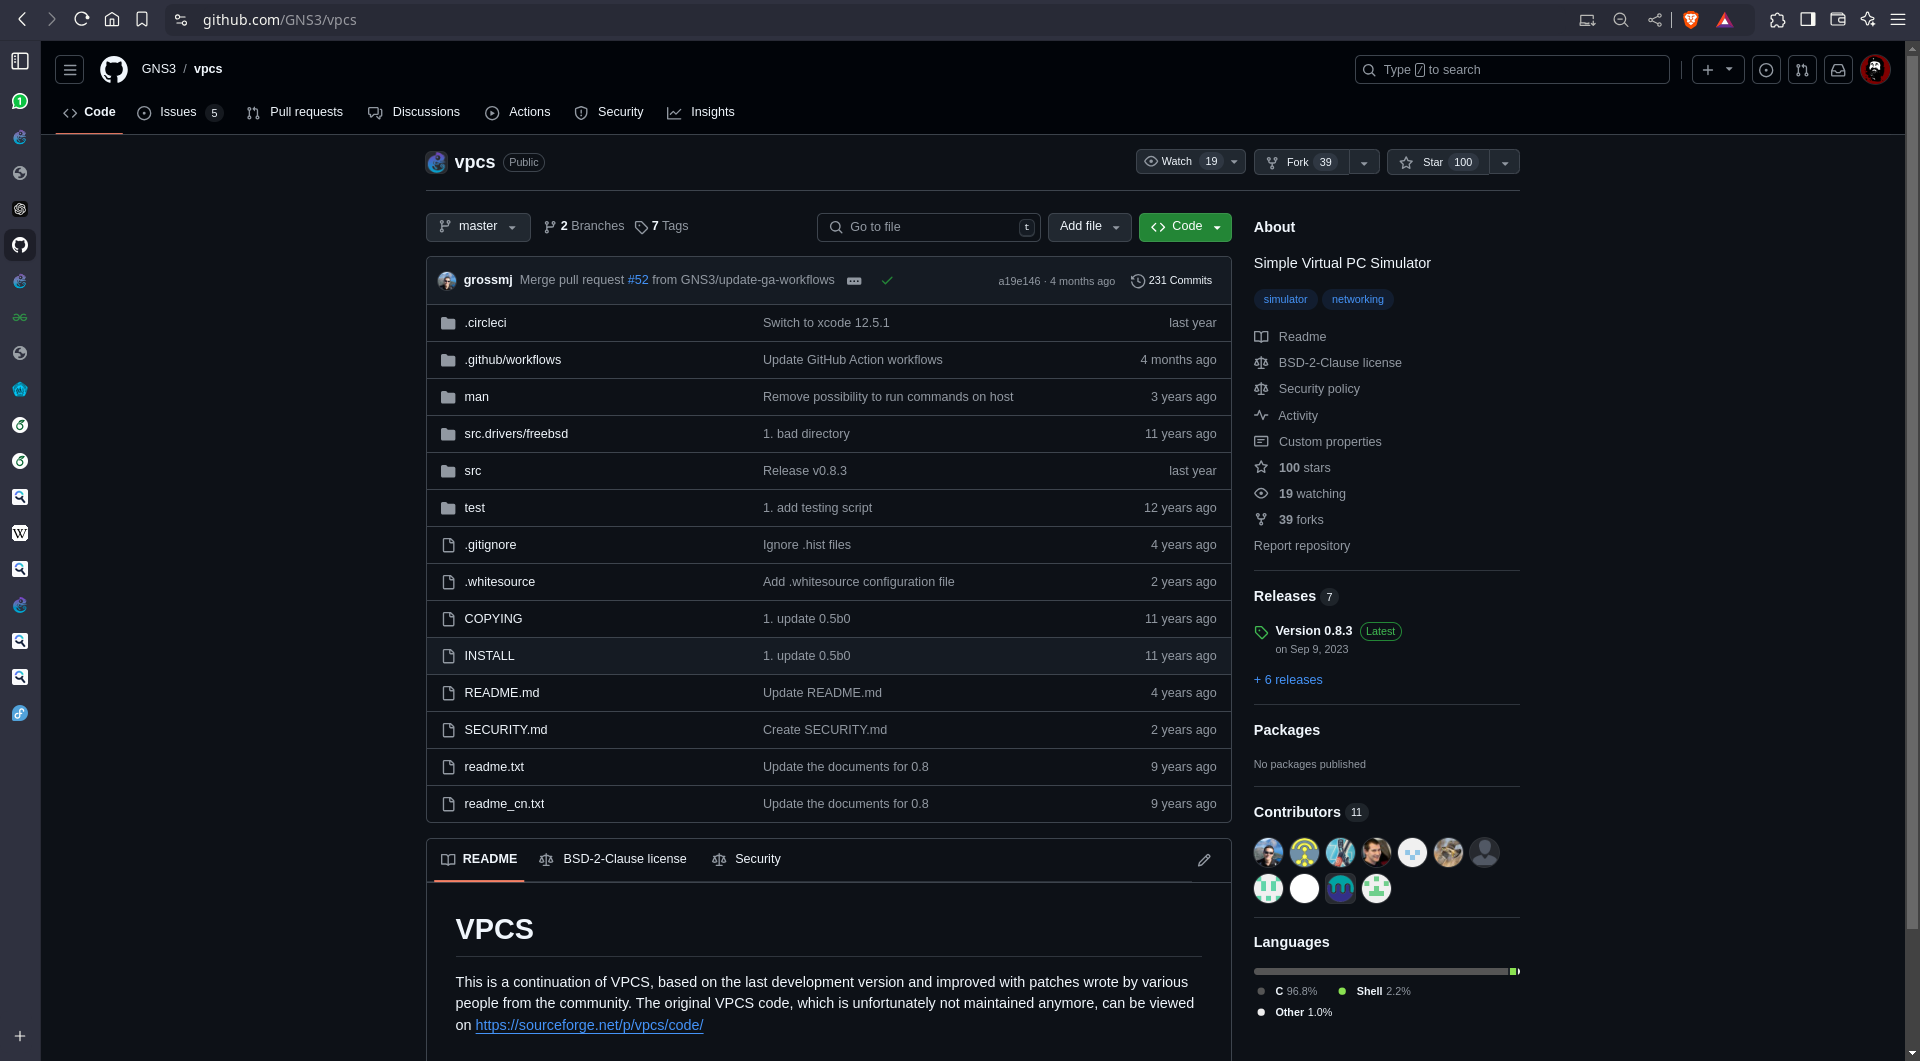
\includegraphics[scale=0.13]{VPCSREPO.png}
              \caption{\small{Halaman Github Project VPCS}}
          \end{figure}

          Lalu dapat diunduh project tersebut melalui opsi download pojok
          kanan atas tepatnya di tombol warna hijau.

          \begin{figure}[h]
              \centering
              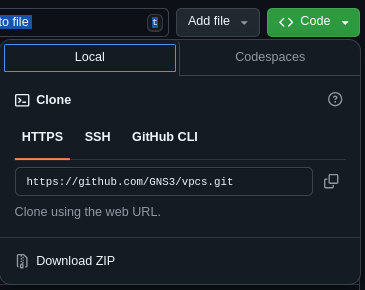
\includegraphics[scale=0.5]{DOWNLOADMENUGIT.png}
              \caption{\small{Opsi Download Repository}}
          \end{figure}

          Atau dengan menggunakan terminal, yaitu dengan perintah git jika telah
          diinstall sebelumnya.

          \$ git clone https://github.com/GNS3/vpcs

          Setelah project telah diinstal, maka perlu dilakukan langkah berikutnya
          yaitu untuk meng-compile program vpcs.

          Tapi sebelum memulai proses kompilasi perlu dipastikan aplikasi-aplikasi
          yang diperlukan seperti kompiler, dan lain sebagainya telah diinstall,
          di fedora linux dapat menggunakan perintah terminal sebagai berikut.

          \$ sudo dnf group install "C Development Tools and Libraries" "Development Tools"

          Lalu setelah menginstall alat-alat yang dibutuhkan, dapat memulai
          proses kompilasi.

          Pertama lakukan 'cd' atau change directory ke dalam folder project
          vpcs yang telah diunduh.

          \$ cd vpcs

          jika dilakukan dengan benar, maka sekarang working directory terminal
          akan berada di dalam folder project vpcs, untuk memastikan dapat
          di lampirkan isi dari folder project tersebut dengan perintah.

          \$ ls -l

          \begin{figure}[h]
              \centering
              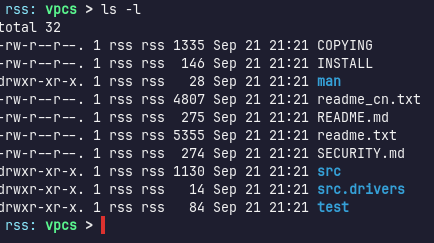
\includegraphics[scale=0.3]{VPCSDIRLS.png}
              \caption{\small{Isi Folder Project VPCS}}
          \end{figure}


          Selanjutnya, 'cd' lagi kedalam folder yang bernama 'src', dengan perintah
          yaitu.

          \$ cd src

          Jika dilakukan perintah 'ls' atau list directory kembali didalam
          folder 'src' ini akan terlihat bahwa folder ini berisikan file-file
          source code dan juga sebuah file script yang executable untuk membuat
          executable vpcs, yaitu 'mk.sh'.


          \begin{figure}[h]
              \centering
              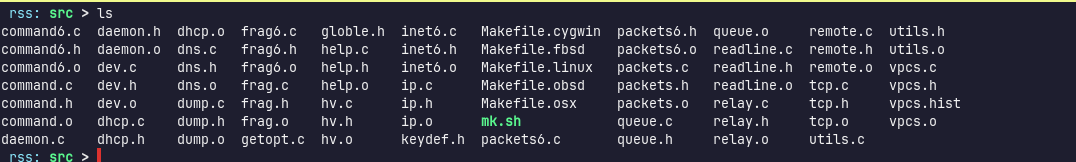
\includegraphics[scale=0.3]{VPCSSRCDIRLS.png}
              \caption{\small{Isi Folder 'src' Project VPCS}}
          \end{figure}


          Yang hanya perlu dilakukan sekarang adalah untuk menjalankan
          script tersebut, didalam terminal ini dapat dilakukan dengan.

          \$ sh mk.sh

          \begin{figure}[h]
              \centering
              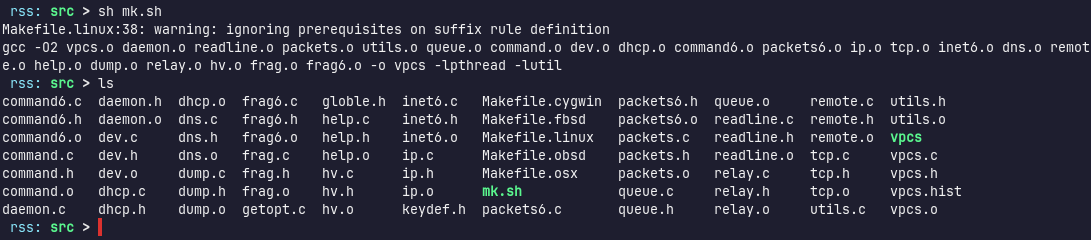
\includegraphics[scale=0.3]{VPCSBUILD.png}
              \caption{\small{Hasil Proses Kompilasi}}
          \end{figure}

          Setelah berhasil untuk di kompile, maka selanjutnya hanya untuk
          meletakan executable vpcs ini di tempat yang sesuai, biasanya
          sistem linux menaruh file-file executable di dua tempat yaitu
          di /usr/bin untuk user root atau admin, dan untuk user di
          .local/bin di path home masing-masing user biasa.

          Jika semua itu telah dilakukan maka GNS-3 akan dapat menemukan executable
          tersebut.

        \item VirtualBox dan QEMU

          John C. Neumann dalam bukunya menjelaskan bahwa VirtualBox adalah.
          ``\emph{VirtualBox is a powerful x86 and AMD64/Intel64 virtualization
          product for enterprise as well as home use. With VirtualBox,
          users can create and manage virtual machines that run various operating
          systems, allowing for complex network topologies and scenarios to be simulated w
          ithin GNS3. This flexibility enables users to test different
          environments and configurations effectively}`` (Neumann, 2021).

          Dan ia juga menjelaskan tentang QEMU, bahwa QEMU adalah.
          ``\emph{QEMU is an open-source machine emulator and virtualizer that enables
          users to run operating systems and applications for different hardware
          architectures. In the context of GNS3, QEMU provides the ability to emulate
          various types of devices and create a more comprehensive simulation of network
          environments. It is particularly useful for integrating virtual machines into
          complex network topologies, facilitating detailed testing and analysis}`` (Neumann, 2021).
          VirtualBox dan QEMU adalah aplikasi untuk membuat mesin-mesin komputer
          virtual untuk diletakan dalam topologi jaringan di GNS-3.

          Kesimpulannya VirtualBox dan QEMU akan digunakan gns-3 untuk
          nantinya mengatur berbagai mesin komputer virtual didalam
          sistem jaringan yang ia simulasikan, dan dapat digunakan
          oleh kita untuk membuat mesin virtualisasi secara mudah.

          Didalam Fedora Linux, untuk menginstall VirtualBox serta QEMU dapat dengan 
          mudah melalui repository fedora linux, dengan perintah terminal yaitu.

          \$ sudo dnf install VirtualBox QEMU

      \end{enumerate}

    \newpage
    \subsection{Membangun Sebuah Topologi Jaringan Sederhana dengan GNS-3}

      Di bagian akan didemonstrasikan bagaimana cara membangun sebuah topologi
      jaringan menggunakan GNS-3.

      Topologi yang akan dibangun disini adalah topologi bintang atau star,
      dalam topologi ini akan dibutuhkan sebuah router dimana beberapa komputer
      akan tersambung hingga dapat berkomunikasi antara satu sama lainnya.

      \begin{figure}[h]
          \centering
          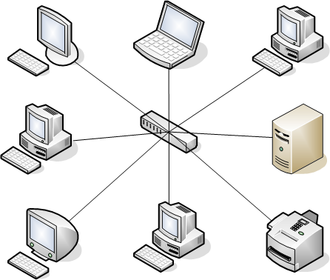
\includegraphics[scale=0.4]{StarTopologi.png}
          \caption{\small{Ilustrasi Topologi Bintang }}
      \end{figure}

      Dalam topologi yang hendak dibuat, akan digunakan setidaknya dua vm linux
      dan juga dua  VPCS untuk bertindak sebagai dua komputer lainnya, serta router yang akan
      digunakan adalah router default yang ada di GNS-3, switch yang disediakan
      GNS-3 ini tidak akan memiliki fitur khusus dan hanya dapat menghubungkan
      antara beberapa device sekaligus.

      Di GNS-3 juga dapat menambahkan router, switch, atau hub bermerk Cisco,
      Mikrotik atau yang serupa, namun memerlukan image software yang berjalan
      didalam mesin-mesin tersebut.

      \newpage 
      Langkah pertama yang perlu dilakukan adalah untuk membuat project baru di
      dalam GNS-3. Ketika pertama kali membuka aplikasi GNS-3, biasanya akan
      terlihat window seperti ini.

      \begin{figure}[h]
          \centering
          \includegraphics[scale=0.13]{GNS3\_CREATEPROJECT.png}
          \caption{\small{Window Membuat Project}}
      \end{figure}

      Didalam window tersebut akan terlihat beberapa hal yang bisa diisi, seperti
      nama project dan letak dimana project akan di simpan.

      Disarankan untuk menggunakan nama project yang deskriptif agar dapat
      dengan mudah dikenali.

      Jika tampilan window ini tidak muncul, dapat juga melalui tombol "file"
      di pojok kiri atas, lalu pilih opsi untuk membuat project baru.

      Setelah membuat project, baru workspace dan bagian-bagian dapat digunakan.


      Langkah selanjutnya adalah untuk meletakan node-node kedalam workspace,
      untuk melihat device apa saja yang tersedia dapat dibuka menu End Device,
      pada Device Toolbar, menu ini di representasikan dengan logo komputer.

      \begin{figure}[h]
          \centering
          \includegraphics[scale=0.12]{GNS3\_SELTOOLBAR.png}
          \caption{\small{Membuka menu End Devices}}
      \end{figure}

      Setelah icon tersebut ditekan, dapat terlihat menu sebagai berikut.

      \begin{figure}[h]
          \centering
          \includegraphics[scale=0.10]{GNS3\_ENDDEVMENU.png}
          \caption{\small{Tampilan Menu End Devices}}
      \end{figure}

      Di menu ini akan terlihat beberapa device yang akan digunakan, untuk
      demonstrasi ini hanya akan digunakan device VPCS dan dua mesin virtual
      yang telah diinstal didalam VirtualBox.

      Untuk menambahkan sebuah node, dapat dilakukan dengan meng-click dan drag
      cursor diatas icon device yang ingin ditambahkan, lalu letakan didalam 
      workspace.

      \begin{figure}[h]
          \centering
          \includegraphics[scale=0.10]{GNS3\_VPCSPLACED.png}
          \caption{\small{Dua Mesin VPCS didalam Workspace}}
      \end{figure}

      Setelah menambahkan kedua VPCS tersebut maka yang perlu dilakukan berikutnya
      adalah menambahkan mesin-mesin VirtualBox kedalam GNS-3, yang dapat dilakukan
      dengan sebagai berikut.

      Pertama buka menu setting yang terletak pada toolbar kiri atas, yang
      bertulisan "Edit", lalu buka menu Preffrence.

      \begin{figure}[h]
          \centering
          \includegraphics[scale=0.10]{GNS3\_SETTINGWINDOW.png}
          \caption{\small{Menu Pengaturan GNS-3}}
      \end{figure}

      Dalam menu ini dapat dilihat beberapa opsi konfigurasi GNS-3, namun untuk
      menambahkan mesin VirtualBox, buka menu "VirtualBox VMs" yang terletak
      pada tab VirtualBox.

      \begin{figure}[h]
          \centering
          \includegraphics[scale=0.13]{GNS3\_VIRTBOXMENU.png}
          \caption{\small{Menu Pengaturan VirtualBox GNS-3}}
      \end{figure}


      Setelah membuka menu tersebut, tekan tombol yang bertuliskan "new", ini
      akan menampilkan menu untuk menambahkan mesin virtual VirtualBox kedalam
      GNS-3. Jangan lupa untuk menekan tombol "Apply" agar konfigurasi
      tersimpan.

      \begin{figure}[h]
          \centering
          \includegraphics[scale=0.13]{GNS3\_ADDVM.png}
          \caption{\small{Menu Penambahan Mesin VirtualBox}}
      \end{figure}

      Setelah memilih mesin VM untuk ditambahkan tekan tombol finish, lalu
      mesin virtual tersebut akan ditampilkan didalam menu "End Devices" yang
      telah dibuka sebelumnya.

      \begin{figure}[h]
          \centering
          \includegraphics[scale=0.10]{GNS3\_IMPORTEDVM.png}
          \caption{\small{Workspace dengan Mesin Virtual VirtualBox}}
      \end{figure}

      Dengan semua VPCS dan Mesin Virtual telah ditambahkan, sekarang yang
      perlu ditambahkan adalah sebuah switch yang akan menghubungkan semua device 
      tersebut kedalam jaringan yang sama.

      Untuk menambahkan sebuah switch cukup mirip dengan menambah device seperti
      sebelumnya, semua opsi device terletak didalam Device Toolbar. Tepatnya
      didalam menu device router dapat dibuka dengan sebagi berikut.

      \begin{figure}[h]
          \centering
          \includegraphics[scale=0.15]{GNS3\_SWITCHMENU.png}
          \caption{\small{Icon Menu Device Switch}}
      \end{figure}

      Setelah ditekan ikon tersebut maka akan terlihat sepert menu "End Devices"
      Sebelumnya, hanya saja disini akan hanya terlihat device-device router atau
      switch dan lain sebagainya.

      Lakukan yang sama untuk menambahkan device VPCS dan letakan sebuah switch
      kedalam workspace GNS-3.
 
      \begin{figure}[h]
          \centering
          \includegraphics[scale=0.10]{GNS3\_ADDSWITCH.png}
          \caption{\small{Workspace dengan Semua Device}}
      \end{figure}    

      \newpage

      Sekarang semua device telah diletakan kedalam workspace, namun semua device
      ini belum terhubung dengan satu sama lain.

      Untuk menghubungkan device-device tersebut dapat menggunakan sebuah tool,
      yaitu dengan menekan tombol "add-a-link" yang terletak pada Toolbar Devices,
      ikon yang digunakan berbentuk kabel lengkap dengan koneksi RJ-45 nya.

      \begin{figure}[h]
          \centering
          
\includegraphics[scale=0.8]{ADDALINKICON.png}
          \caption{\small{Icon Tombol "add-a-link"}}
      \end{figure}    

      Setelah tombol tersebut ditekan, maka akan berubah menjadi sebagai berikut,
      yang menandakan sekarang anda dapat menghubungkan device.

      \begin{figure}[h]
          \centering
          
\includegraphics[scale=0.2]{ADDALINKPRESSEDICON.png}
          \caption{\small{Icon Tombol "add-a-link" Ditekan}}
      \end{figure}    

      Sekarang untuk tiap device yang dibuat, hubungkan tiap mesin dengan 
      switch yang dibuat tadi hingga terhubung sebagai berikut.

      \begin{figure}[h]
          \centering
          \includegraphics[scale=0.1]{GNS3\_CONNECTED.png}
          \caption{\small{Semua Device terhubung menggunkanan Topologi Bintang}}
      \end{figure}    

      \newpage

      Selanjutnya yang perlu dilakukan adalah mengkonfigurasi IP semua device
      agar dapat saling berkomunikasi.

      Untuk merubah konfigurasi IP pada device VPCS dapat dilakukan dengan
      membuka console device nya lalu dengan perintah yaitu, 
      "ip <ip yang ingin digunakan>".

      Berikut adalah konfigurasi IP pada device "PC1" dan "PC2".

      \begin{figure}[h]
          \centering
          \includegraphics[scale=0.3]{PC1\_IPCONF.png}
          \caption{\small{Konfigurasi IP PC1}}
      \end{figure}    

      \begin{figure}[h]
          \centering
          \includegraphics[scale=0.3]{PC2\_IPCONF.png}
          \caption{\small{Konfigurasi IP PC2}}
      \end{figure}    

      Setelah mengkonfigurasi IP dari kedua VPCS tersebut sekarang kedua VM
      yang terhubung pun harus diberikan IP Statis.

      \newpage

      Berikut konfigurasi kedua VM tersebut.

      \begin{figure}[h]
          \centering
          \includegraphics[scale=0.3]{XUBUNTU\_IPCONF.png}
          \caption{\small{Konfigurasi IP Xubuntu}}
      \end{figure}    

      \begin{figure}[h]
          \centering
          \includegraphics[scale=0.3]{KALI\_IPCONF.png}
          \caption{\small{Konfigurasi IP Kali Linux}}
      \end{figure}    

      \begin{figure}[h]
          \centering
          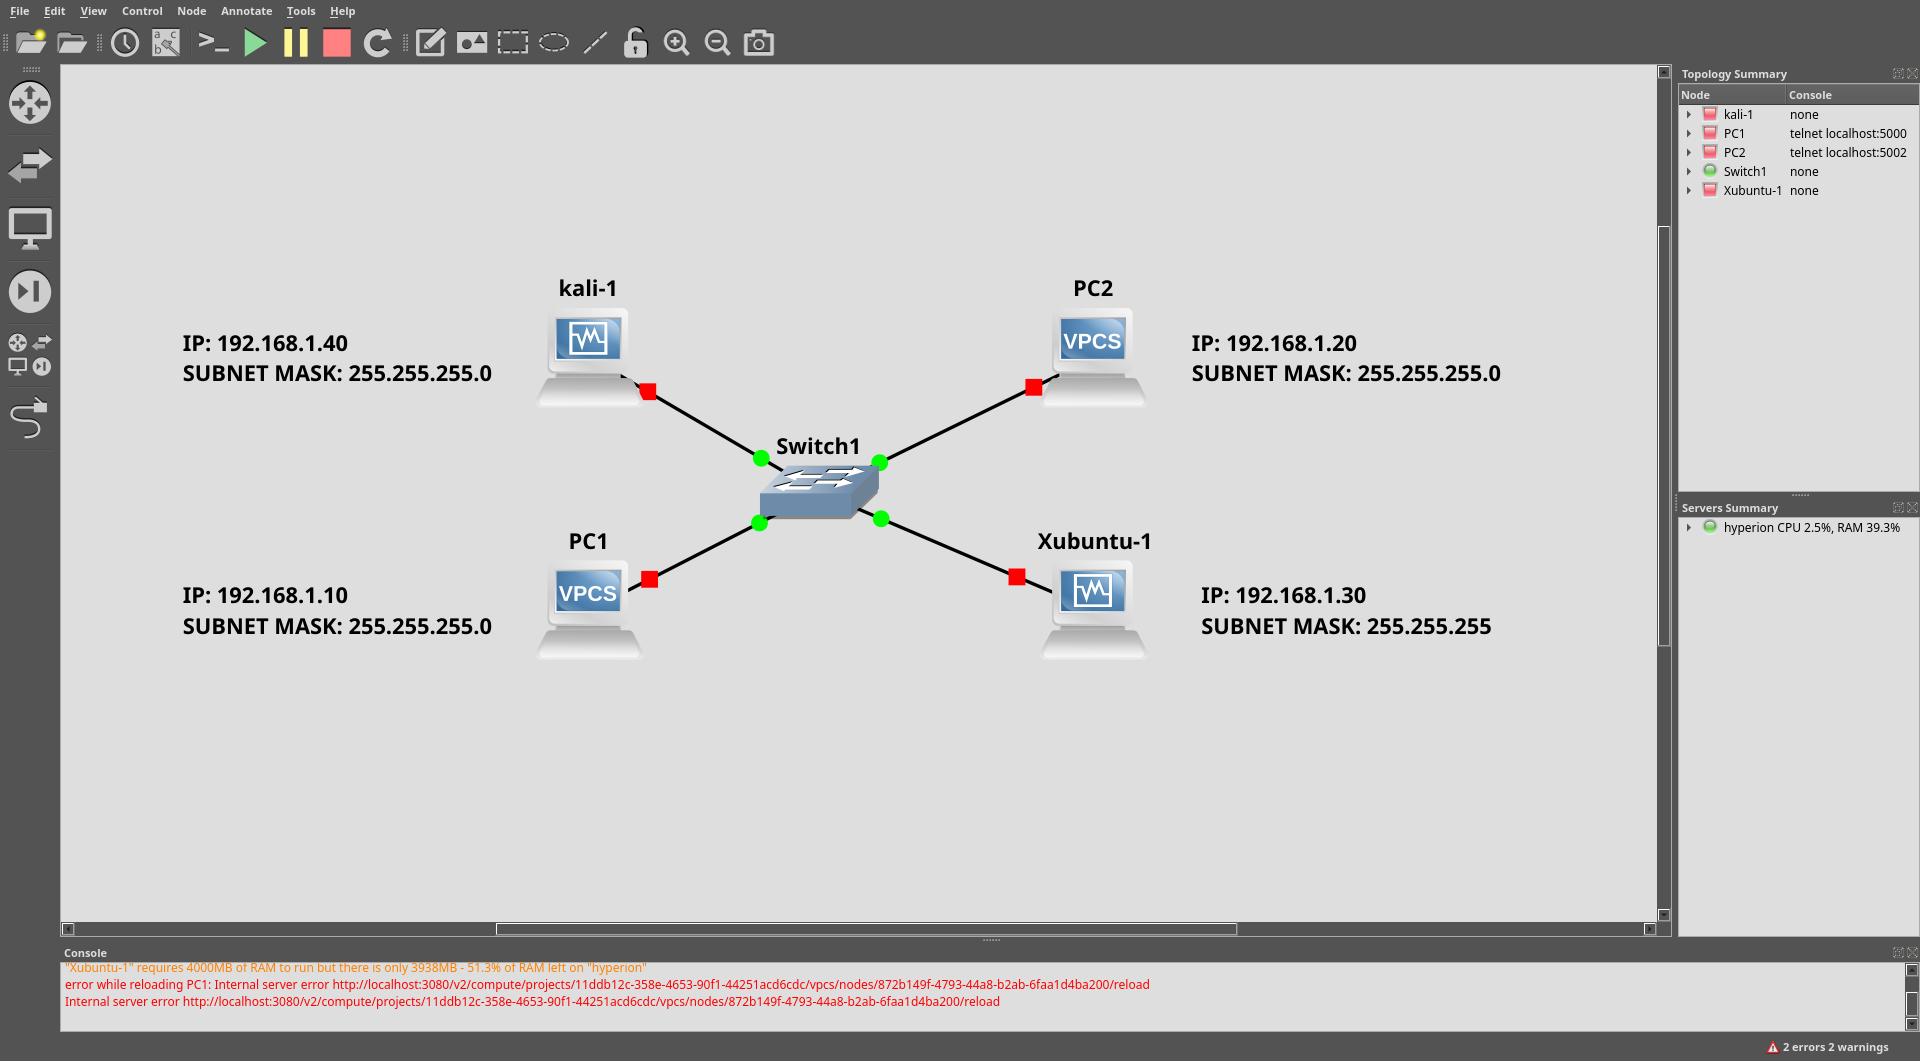
\includegraphics[scale=0.12]{GNS3_DevicesIP.png}
          \caption{\small{Konfigurasi IP Semua Device}}
      \end{figure}    

      Dengan semua device telah diberikan alamat IP masing-masing, yang
      perlu dilakukan selanjutnya adalah untuk menguji apakah device yang
      ada pada simulasi ini dapat saling komunikasi.

      \newpage

      Pengujian sederhana dapat dilakukan menggunakan perintah yang bernama "ping".
      Perintah "ping" akan ada didalam konsole VPCS dan juga VM Linux yang digunakan disini.
      Perintah ini akan mengirim data packet ke IP yang dituju.
      Berikut adalah beberapa hasil pengujian tersebut.

      \begin{enumerate}[label=\arabic*.]

      \item Kali Linux dengan Xubuntu

          \begin{figure}[h]
              \centering
              \includegraphics[scale=0.4]{KALI\_PINGOUT.png}
              \caption{\small{Hasil Output Ping Dari VM Kali Linux ke VM Xubuntu}}
          \end{figure}    

          Disini terdapat beberapa hal yang perlu dicermati, pertama yang
          ditunjuk oleh panah "1", itu adalah perintah terminal yang digunakan,
          perintah tersebut mengatakan untuk mengirim packet sebanyak lima kali
          ke alamat IP "192.168.1.30", yaitu alamat IP Xubuntu.

          Panah "2" dan "3" menunjukan output dari perintah ping ini, dengan panah
          "3", memberikan informasi tentang keberhasilan pengiriman
          packet-packet tersebut.

      \item PC1 dengan PC2

      \begin{figure}[h]
          \centering
          \includegraphics[scale=0.5]{PC1\_PINGOUT.png}
          \caption{\small{Hasil Output Ping Dari VPCS PC1 ke VPCS PC2}}
      \end{figure}    

        Output ping dari konsole VPCS menunjukan PC1 dan PC2 dapat saling
        berkomunikasi.

      \newpage
      \item Kali Linux dengan PC1

      \begin{figure}[h]
          \centering
          \includegraphics[scale=0.3]{KALI\_PINGOUT2.png}
          \caption{\small{Hasil Output Ping Dari VM Kali Linux ke VPCS PC1}}
      \end{figure}    

          Disini dapat dilihat semua packet berhasil dikirimkan, menandakan
          VM Kali Linux ini dengan VPCS PC1 dapat saling berkomunikasi.

      \item PC2 dengan Xubuntu

      \begin{figure}[h]
          \centering
          \includegraphics[scale=0.5]{PC2\_PINGOUT.png}
          \caption{\small{Hasil Output Ping Dari VPCS PC2 ke VM Xubuntu}}
      \end{figure}    

          Disini dapat dilihat semua packet berhasil dikirimkan, menandakan
          VPCS PC2 ini dengan VM Xubuntu dapat saling berkomunikasi.

      \end{enumerate}

      Maka, dengan semua device dalam topologi dapat saling berkomunikasi dapat
      disimpulkan bahwa dalam demonstrasi ini telah diperlihatkan langkah-langkah
      untuk membangun sebuah sistem jaringan komputer yang sederhana, dengan
      semuanya dilakukan dengan bantuan GNS-3.

  \newpage

  \begin{center}
    \large{\textbf{BAB III}}

    \section*{KESIMPULAN}
  \end{center}
  \addcontentsline{toc}{section}{BAB III KESIMPULAN}{}

  \vspace{1cm}

  Dari laporan ini, dapat disimpulkan bahwa aplikasi GNS-3 adalah aplikasi wajib
  bagi siapapun yang ini mempelajari Jaringan Komputer, dan tentunya yang ingin
  memiliki karier dibidang jaringan.

  Dan bagi seorang mahasiswa, aplikasi ini menyediakan kesempatan untuk berkesperimen
  dan bereksplorasi seputar jaringan komputer, dan tentunya tanpa harus memikirkan
  tentang biaya tambahan untuk membangun sebuah sistem jaringan fisik.

  \newpage

  \begin{center}
    \section*{DAFTAR PUSTAKA}
  \end{center}
  \addcontentsline{toc}{section}{DAFTAR PUSTAKA}{}
  \vspace{1cm}

\begin{enumerate}
  \item Ambarwati, S., \& Fauzi, A. (2019). Jaringan komputer dan telekomunikasi. Andi Publisher.
  \item Neumann, J. C. (2021). The book of GNS3. O'Reilly Media.
\end{enumerate}



\end{document}
